\cite{Viola01rapidobject} osmislili su prvi algoritam za detekciju objekata koji je radio u stvarnom vremenu. Originalno je razvijen za detekciju lica, ali moguće ga je trenirati za detekciju bilo koje vrste objekata. Tri novosti koje je algoritam donio u odnosu na prijašnje algoritme su novi način prikaza slike, algoritam za učenje temeljen na AdaBoostu i kombiniranje više klasifikatora u kaskadu počevši od jednostavnijih prema složenijima.

Algoritam radi tako da klizeći prozor prolazi po slici i za svaki prozor određuje nalazi li se objekt u njemu. Nakon svakog prolaza cijele slike prozor se povećava za određeni faktor i postupak se ponavlja. Faktor povećanja prozora direktno utječe na performanse algoritma tako da se povećanjem faktora smanjuje vrijeme potrebno za obradu jedne slike, ali se time može pogoršati preciznost i, suprotno, smanjenjem faktora se povećava vrijeme potrebno za obradu slike, ali se preciznost detekcije može povećati.
Klasifikatori ne rade s pikselima, nego sa značajkama jer se značajkama lakše može opisati domensko znanje koje bi bilo teško naučiti iz piksela. Algoritam koristi tri vrste značajki: značajke s dva, tri i četiri pravokutnika. Značajke s dva pravokutnika se računaju tako da se unutar slike izaberu dva susjedna pravokutnika jednakih veličina, a vrijednost značajke je razlika sume piksela dvaju pravokutnika. Analogno tome se računaju i značajke s tri i četiri pravokutnika. Primjeri značajki su prikazani na slici \ref{viola-jones-znacajke}.
Navedene značajke se mogu izračunati u konstantnom vremenu ako se slika prikazuje kao integralna slika. Integralna slika na lokaciji $x, y$ sadrži sumu piksela iznad i lijevo od te točke, uključujući i tu točku. Vrijednost integralne slike na lokaciji $x, y$ je opisana formulom:
\[
	ii(x, y) = \sum\limits_{x' \leq x, y' \leq y} i(x', y')
\]
, gdje je $ii(x, y)$ integralna slika, a $i(x, y)$ originalna slika. Integralna slika se iz originalne slike može izračunati u linearnoj vremenskoj složenosti. Koristeći navedeni prikaz slike, suma piksela bilo kojeg pravokutnika unutar slike se može odrediti dohvaćanjem najviše četiri vrijednosti. Primjer izračuna sume piksela unutar pravokutnika prikazan je na slici \ref{viola-jones-pravokutnici}. Ukupan broj značajki koji se može dobiti opisanim postupkom za svaki prozor veličine $24 \times 24$ je veći od $160.000$ što je puno veće od broja piksela u prozoru. Iako je izračunavanje jedne značajke jeftina operacije, izračunavanje svih značajki je skupo i nije praktično za rad u stvarnom vremenu. Pretpostavka algoritma, koja je potvrđena eksperimentima, je da se mali podskup značajki može iskoristiti za izgradnju dobrog klasifikatora. Za odabir podskupa značajki i treniranje klasifikatora koristi se varijanta algoritma AdaBoost.

\begin{lstlisting}
Pseudokod algoritma AdaBoost:
  - Skup podataka za trening s n primjera $(x_1, y_1),...,(x_n, y_n)$,
    gdje je $y_i=0$ za negativne primjere, a $y_i=1$ za pozitivne
  - Inicijaliziraj: $w_{1, i}=\frac{1}{2m}$ za $y_i = 0$ i $w_{1, i}=\frac{1}{2l}$ za $y_i = 1$,
    gdje je $m$ broj negativnih primjera, a $l$ broj pozitivnih
  - ZA $t = 1,...,T$:
      1. Normaliziraj težine tako da $w_t$ bude vjerojatnosna 
         razdioba: $w_{t, i} \gets \frac{w_{t, i}}{\sum\limits_{j=1}^{n} w_{t,j}}$
      2. Za svaku značajku j, treniraj klasifikator $h_j$ koji
         koristi samo jednu značajku. Greška se računa kao:
           $\epsilon _j = \sum\limits_i w_i|h_j(x_i) - y_i| $
      3. Izaberi klasifikator $h_t$ s najmanjom greškom $\epsilon _t$
      4. Ažuriraj težine:
           $w_{t+1, i} = w_{t, i} \beta _t^{1-e_i}$
         gdje je $e_i = 0$ ako je $x_i$ točno klasificiran,
         a $e_i = 1$ inače i $\beta _t = \frac{\epsilon _t}{1 - \epsilon _t}$
  - Konačni klasifikator je:
\end{lstlisting}
\[
	h(x) = 
	\begin{cases}
	 1, \quad za \quad  \sum\limits_{t=1}^{T} \alpha _t h_t(x) \geq \frac{1}{2} \sum\limits_{t=1}^{T} \alpha _t, \quad \alpha _t = \log{\frac{1}{\beta _t}} \\ 
	 0,	\quad inace
	\end{cases}
\]

Dobiveni klasifikatori se kombiniraju u kaskadu tako da se na početku nalaze jednostavniji klasifikatori koji koriste mali broj značajki, a na kraju složeniji koji za klasifikaciju koriste veći broj značajki. Ako jedan klasifikator prozor označi kao negativan, tj. odredi da se u njemu ne nalazi traženi objekt, prozor se odbacuje i ne prolazi kroz složenije klasifikatore. Ako, s druge strane, klasifikator označi prozor kao pozitivan, on se prosljeđuje sljedećem, složenijem klasifikatoru. Ako su svi klasifikatori označili prozor kao pozitivan, zaključujemo da se traženi objekt nalazi u tom prozoru. Opisani postupak skiciran je na slici \ref{viola-jones-kaskada}. Ideja povezivanja klasifikatora u kaskadu je da jednostavniji klasifikatori odbace veći broj prozora za koje se lako može odrediti da ne sadrže traženi objekt te se time smanji ukupni broj značajki koje je potrebno izračunati. Samo se prozori za koje nije moguće na temelju manjeg broja značajki odrediti da ne sadrže objekt prosljeđuju složenijim klasifikatorima kako bi se postigla veća točnost. Time se postiže ravnoteža između brzine izvođenja i točnosti detekcije.
Za određivanje broja značajki klasifikatora koristi se jednostavan postupak koji se temelji na činjenici da se u kaskadi svakim korakom smanjuje broj lažno pozitivnih primjera i broj detektiranih primjera. Na početku svakog koraka se postavi cilj za minimalno smanjenje lažno pozitivnih primjera i maksimalno smanjenje broja detekcija. Zatim se klasifikator trenira s određenim brojem značajki te mu se dodaju nove značajke sve dok se ne postigne postavljeni cilj. Postupak se ponavlja za svaki klasifikator.
Nakon obrade cijele slike, objekti će uglavnom biti detektirani više puta. Višestruke detekcije se rješavaju tako da se prvo sve detekcije podijele u disjunktne skupove. Dvije detekcije su u istom skupu ako se njihovi prozori preklapaju. Konačna detekcija se dobije tako da se izračuna prosjek koordinata kuteva svih prozora u skupu.

\begin{figure}
	\centering
	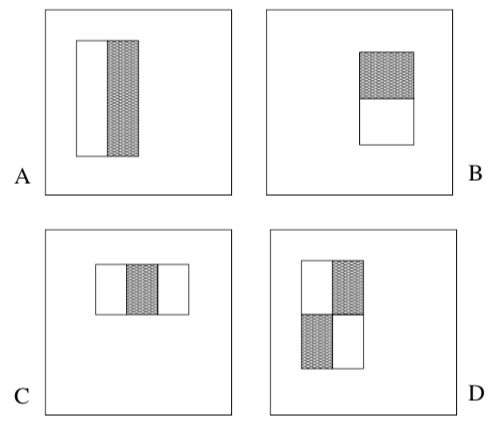
\includegraphics[scale=1]{img/viola-jones-znacajke.png}
	\caption{Primjeri značajki s dva (slike A i B), tri (slika C) i četiri (slika D) pravokutnika. Sume piksela u bijelim pravokutnicima se oduzimaju od sume piksela u sivim pravokutnicima da bi se dobila vrijednost značajke (\cite{Viola01rapidobject}).}
	\label{viola-jones-znacajke}
\end{figure}

\begin{figure}
	\centering
	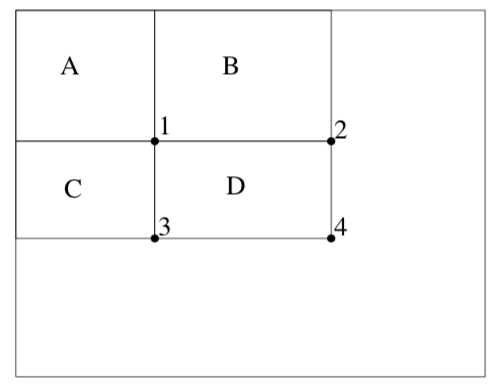
\includegraphics[scale=1]{img/viola-jones-pravokutnici.png}
	\caption{Svaka točka sadrži sumu svih piksela iznad i lijevo od sebe. Točka 1 sadrži sumu piksela unutar pravokutnika A, točka 2 sumu A + B, točka 3 sumu A + C i točka 4 sumu A + B + C + D. Za izračunavanje sume piksela unutar pravokutnika D trebaju nam vrijednosti točaka 1-4 pa sumu možemo izračunati kao $ii(4)$ - ii(3) - ii(2) + ii(1) (\cite{Viola01rapidobject}).}
	\label{viola-jones-pravokutnici}
\end{figure}

\begin{figure}
	\centering
	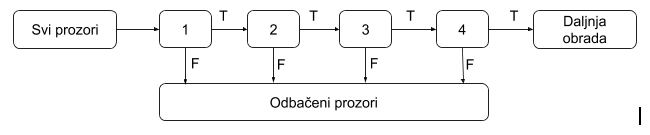
\includegraphics[scale=0.6]{img/viola-jones-kaskada.png}
	\caption{Shematski prikaz kaskade klasifikatora. Klasifikatori su označeni brojevima 1-4 i poredani po složenosti gdje je klasifikator 1 najjednostavniji, a klasifikator 4 najsloženiji. Prozor se odbacuje ako ga bilo koji klasifikator označi kao negativnog.}
	\label{viola-jones-kaskada}
\end{figure}